\documentclass[a4paper]{article}

% Packages
\usepackage[left=25mm, top=30mm,]{geometry}
\usepackage{graphicx}
\usepackage{float}
\usepackage{siunitx}
\usepackage{listings}
\usepackage{physics}
\usepackage[dutch]{babel}


\usepackage{hyperref}
\hypersetup{pdfborder={0 0 0}}

% Commands and stuff
\newcommand{\opgave}[1]{\subsection{Opgave #1}}

% Title Page stuff
\title{Practicum Numerieke Modelering en Benadering}
\author{Wim Kunnen \\ Bo Kleynen}
\date{Vrijdag 6 april 2018 }

% Actual document
\begin{document}

\begin{titlepage}
\maketitle
\thispagestyle{empty}
\end{titlepage}

% Table of Contents
\tableofcontents
\thispagestyle{empty}
\cleardoublepage

\pagenumbering{roman}
\setcounter{page}{1}

% List of figures
\listoffigures
\addcontentsline{toc}{section}{\numberline{} Lijst van Figuren}

% List of Tables
\listoftables
\addcontentsline{toc}{section}{\numberline{} Lijst van Tabellen}
\cleardoublepage


\pagenumbering{arabic}
\setcounter{page}{1}

% PDE stuff
\section{Partial Differential Equations}\label{sec:PDE}
Voor de eerste opgaven werd de Poisson vergelijking numeriek opgelost als randvoorwaarde probleem. Het de implementatie van het algoritme werd in Matlab geschreven en is te vinden op pagina \pageref{sec:pde}.

Vergelijking \ref{eq:poisson} toont de wiskundige formulering van het randvoorwaardeprobleem.
\begin{equation}\label{eq:poisson}
	\pdv[2]{u(x,y)}{x} + \pdv[2]{u(x,y)}{y} = f(x,y) \quad met (x,y) \in D = [ \, 0,1 ]\, \times [ \, 0,1 ]\,
\end{equation}
Met als randen:
\begin{equation}\nonumber
	u_w(y) = u(0,y), \quad u_o = u(1,y), \quad u_z = u(x,0) \quad en \quad u_n = u(x,1)
\end{equation}

% OPGAVE 1
\opgave{1: Implementatie en controle}\label{sec:oef1}
Zoals vermeld in sectie \ref{sec:PDE} werd de Poisson vergelijking \ref{eq:poisson} opgelost aan de hand van de Matlab code op pagina \pageref{sec:pde}.
De implementatie werd getest aan de hand van volgende input vergelijkingen u(x,y):
\begin{equation}\nonumber
	u(x,y) = 1,\quad u(x,y) = 1 + x + y \quad en \quad u(x,y) = x^2 +y^2
\end{equation}
Deze vergelijkingen werden opgelost in het Matlab bestand opgave1.m, te vinden op pagina \pageref{sec:code1}.
Wanneer we handmatig de oplossing vergeleken met de oplossing merkten we dat er bijna geen afwijkingen waren ten opzichte van de gegeven oplossingen. Een exactere test naar de nauwkeurigheid van onze implementatie staat uitgewerkt in sectie \ref{sec:oef2}.

% OPGAVE 2
\opgave{2: Fouten en tijdsduur}\label{sec:oef2}
In deze sectie bekijken we de nauwkeurigheid van onze Matlab implementatie aan de hand van de volgende input vergelijking:
\begin{equation}\nonumber
	u(x,y) = e^{x+y}
\end{equation}
Deze vergelijking werd opgelost in het Matlab script opgave2.m, waarvan de implementatie te vinden is op pagina \pageref{sec:code2}. De discretisatie stap, maximale fout en de tijdsduur voor de berekening werden uitgezet in tabel \ref{tab:fouten}.

% Tabel met fouten
\begin{table}[H]
	\centering
	\begin{tabular}{l c r}
		N & Maximale fout & Tijd [seconde] \\ \hline
		8 & \num{1.6118e-04} & 0.002915 \\
		16 & \num{4.5544e-05} & 0.000922 \\		
		32 & \num{1.2136e-05} & 0.000538 \\
		64 & \num{3.1300e-06} & 0.000827 \\
		128 & \num{7.9485e-07} & 0.005202 \\
		256 & \num{2.0027e-07} & 0.013696 \\
		512 & \num{5.0268e-08} & 0.039208 \\
		1024 & \num{1.2605e-08} & 0.231955
	\end{tabular}
	\caption{Tabel met fouten in functie van discretisatie}
	\label{tab:fouten}
\end{table}

Een voorzichtige schatting leert ons dat de maximale fout $\mathcal{O}(\frac{3}{2}N)$ is.
\cleardoublepage

% OPGAVE 3
\opgave{3: Plot}\label{sec:oef3}
Voor de laatste opgave rond de Poisson vergelijking schreven we een Matlab script dat het volgende randvoorwaardeprobleem oplost. \begin{equation}\nonumber
f(x,y) =
  \begin{cases}
    -100       & \quad \text{als } (x,y) \in D = [ \, 0.4,0.6 ]\, \times [ \, 0.4,0.6 ]\,\\
    0  & \quad \text{anders }
  \end{cases}
\end{equation}
Met randen:
\begin{equation}\nonumber
	u_w(y) = 3, \quad u_o = 2, \quad u_z = 2+\sin{(\frac{\pi}{2}x)} \quad en \quad u_n = 1
\end{equation}

Daarna worden de oplossing (figuur \ref{fig:Plot3}) en de contourlijnen (figuur \ref{fig:Contour3}) geplot. De implementatie wordt gegeven op pagina \pageref{code3}, in de code van opgave3.m.
Voor de plots werd een discretisatiestap van 128 gekozen. Deze waarde werd voldoende groot gekozen voor de nauwkeurigheid van de oplossing, maar niet te groot, aangezien het surf commando het rooster weergeeft en dit nefast was voor het kleurenprofiel van de plot. 

\newpage
% Contour figuur
\begin{figure}[H]
	\begin{center} 
		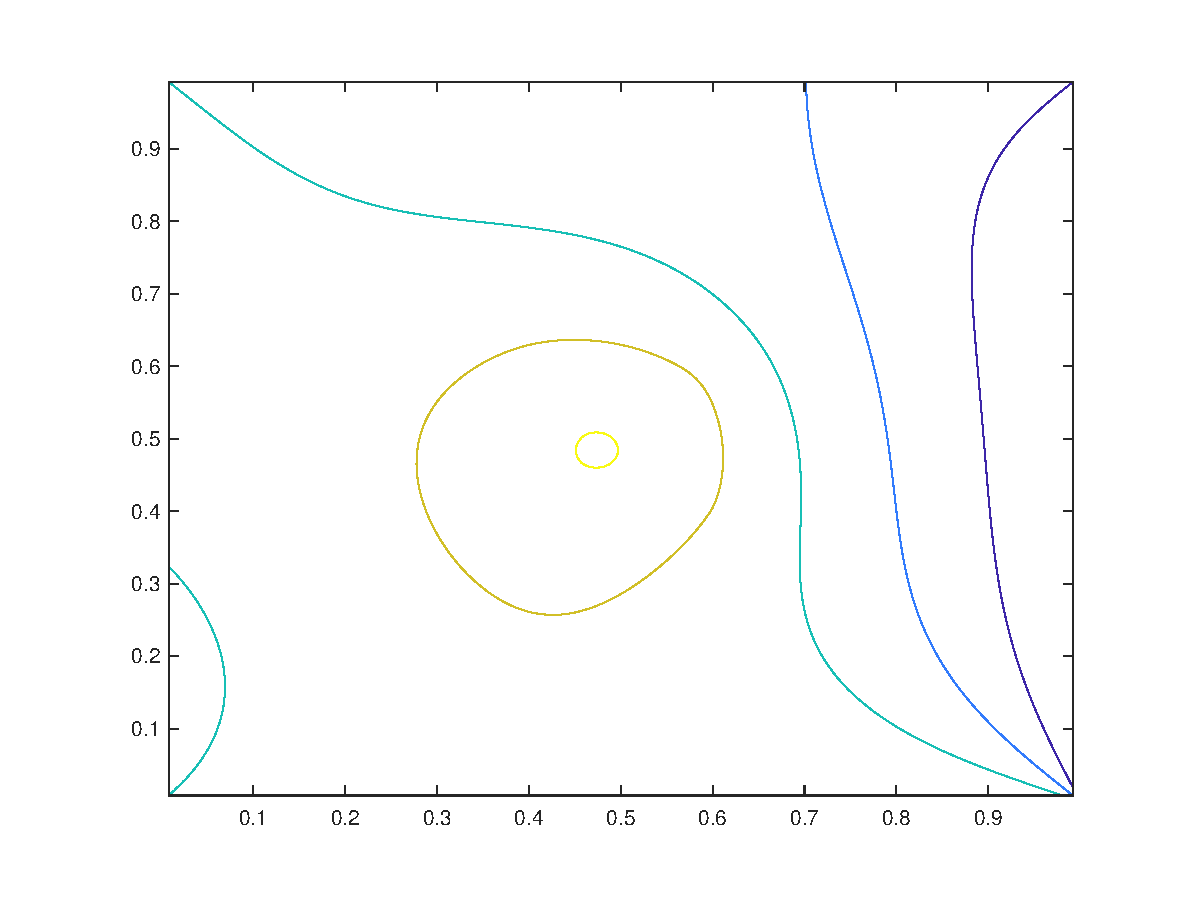
\includegraphics[width=0.7\textwidth]{Contour3.eps}
	\end{center}
	\caption{De contour plot voor Opgave 3.}
	\label{fig:Contour3}
\end{figure}

% Plot
\begin{figure}[H]
	\begin{center} 
		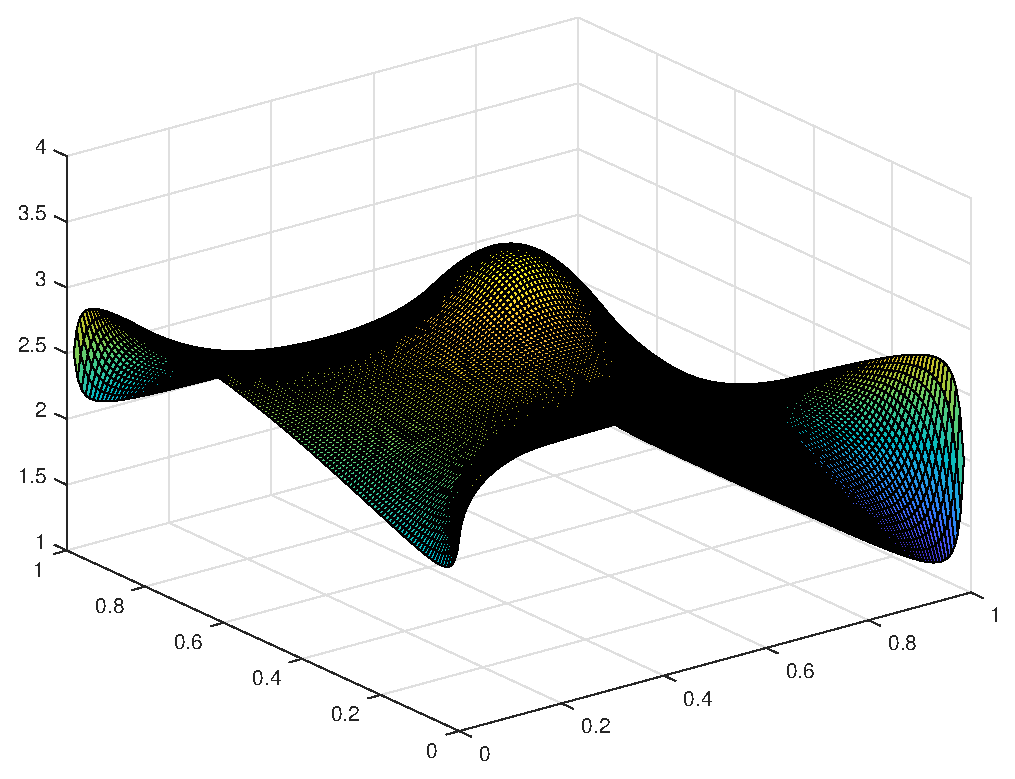
\includegraphics[width=1\textwidth]{Plot3.eps}
	\end{center}
	\caption{De plot voor Opgave 3.}
	\label{fig:Plot3}
\end{figure}
\newpage

% Splines stuff
\section{Splines}\label{sec:splines}
In deze sectie wordt aangetoond dat splines gebruikt kunnen worden voor het oplossen van een kleinste kwadraten benadering (verder als kkb afgekort).

% OPGAVE 4
\opgave{4: Implementatie}\label{sec:oef4}
Voor een effici�nte  evaluatie van B-splines werd het algoritme van de Boor (\ref{eq:deboor}) ge�mplementeerd.
\begin{equation}\label{eq:deboor}
	s(x) = \sum\limits_{i=-k}^{n-1} c_iN_{i, k+1}(x)
\end{equation}
\begin{equation}\label{eq:deboorcoef}
	c_i^{[\, r]\, } = \alpha_{i,r} c_i^{[\, r-1]\, } + (1-\alpha_{i,r})c_{i-1}^{[\, r-1]\, } \quad met \quad \alpha_{i,r} = \frac{x-t_i}{t_{i+k+1-r}-t_i}
\end{equation}
Waarvan de co�ffici�nten bepaald kunnen worden uit (\ref{eq:deboorcoef}).\\
De implementatie van de berekening voor de waarde van een B-spline op een positie x staat gegeven in deBoor.m op pagina \pageref{sec:codedb}.

% OPGAVE 5
\opgave{5: Illustratie correctheid}\label{sec:oef5}
Ter illustratie van de correctheid van het algoritme van de Boor werden 5 kubische splines (graad k = 3) getekend in figuur \ref{fig:splines}.
De Matlab code voor deze tekeningen staat in opgave5.m (pagina \pageref{sec:code5}) en plotBSpline.m (pagina \pageref{sec:codeplotb}).

%Plot Splines
\begin{figure}[H]
	\begin{center} 
		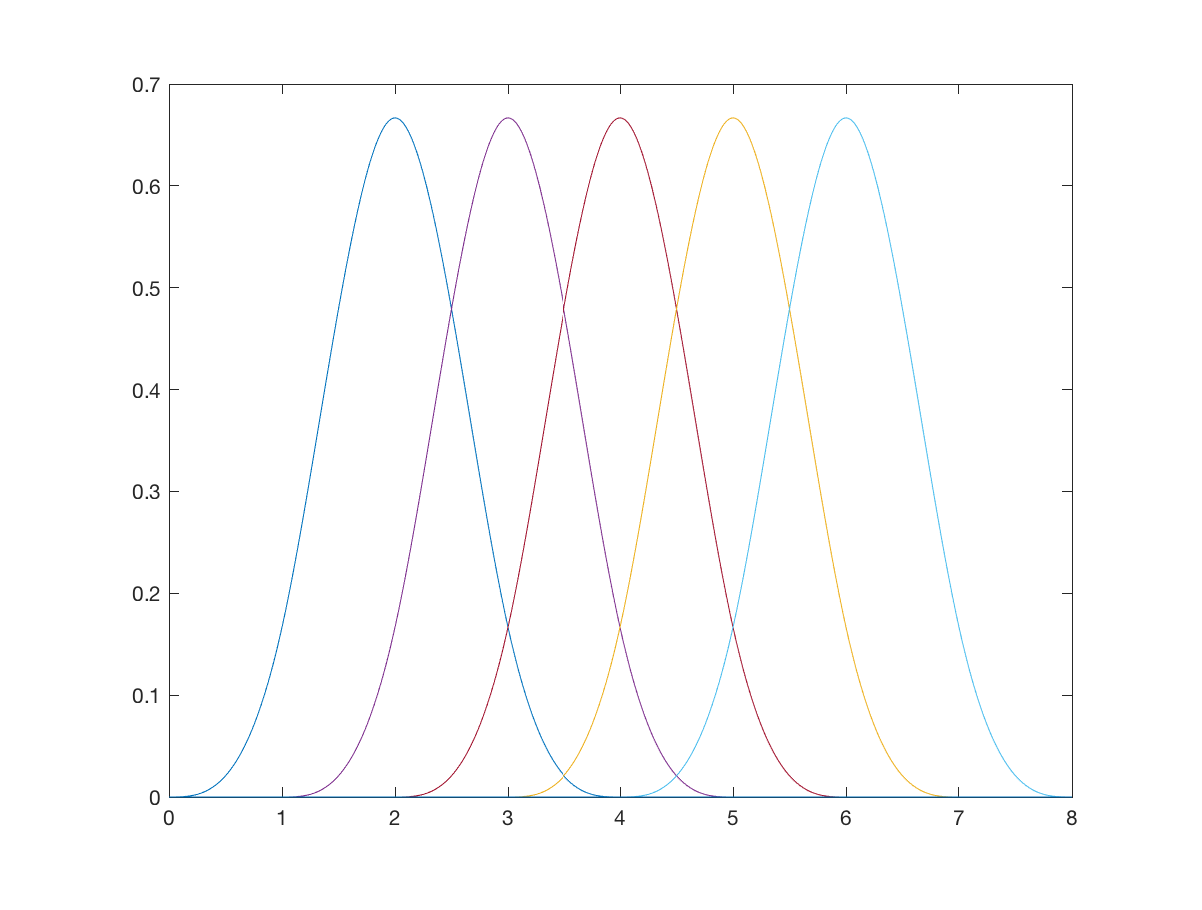
\includegraphics[width=0.6\textwidth]{BSplines.eps}
	\end{center}
	\caption{Kubische B-splines voor Opgave 5.}
	\label{fig:splines}
\end{figure}
\newpage

% OPGAVE 6
\opgave{6: Ligging knooppunten}\label{sec:oef6}

% OPGAVE 7
\opgave{7: Ruis}\label{sec:oef7}
De ruis wordt gemodelleerd aan de hand van (\ref{eq:f}) waaraan een willekeurige component wordt toegevoegd (\ref{eq:noise}).
\begin{equation}\label{eq:f}
	f_{ruis}(x) = \frac{\sin{(20x)}}{100x^2+5}
\end{equation}
\begin{equation}\label{eq:noise}
	f_{ruis}(x) = \frac{\sin{(20x)}}{100x^2+5} + 0.04*randn(size(x))
\end{equation}

Het minimale residu van de benaderingen wordt weergegeven in tabel \ref{tab:splineError}.
%Tabelletje
\begin{table}[H]
	\centering
	\begin{tabular}{l c r}
		Functie & Minimaal residu & Aantal knooppunten \\ \hline
		f(x) & 0.3380 & 199 \\
		Fruis(x) & 0.3469 & 190 \\
	\end{tabular}
	\caption{Optimaal residu en aantal knooppunten}
	\label{tab:splineError}
\end{table}

De code is te vinden in Opgave7.m op pagina \pageref{sec:code7}.

\begin{figure}[H]
	\begin{center} 
		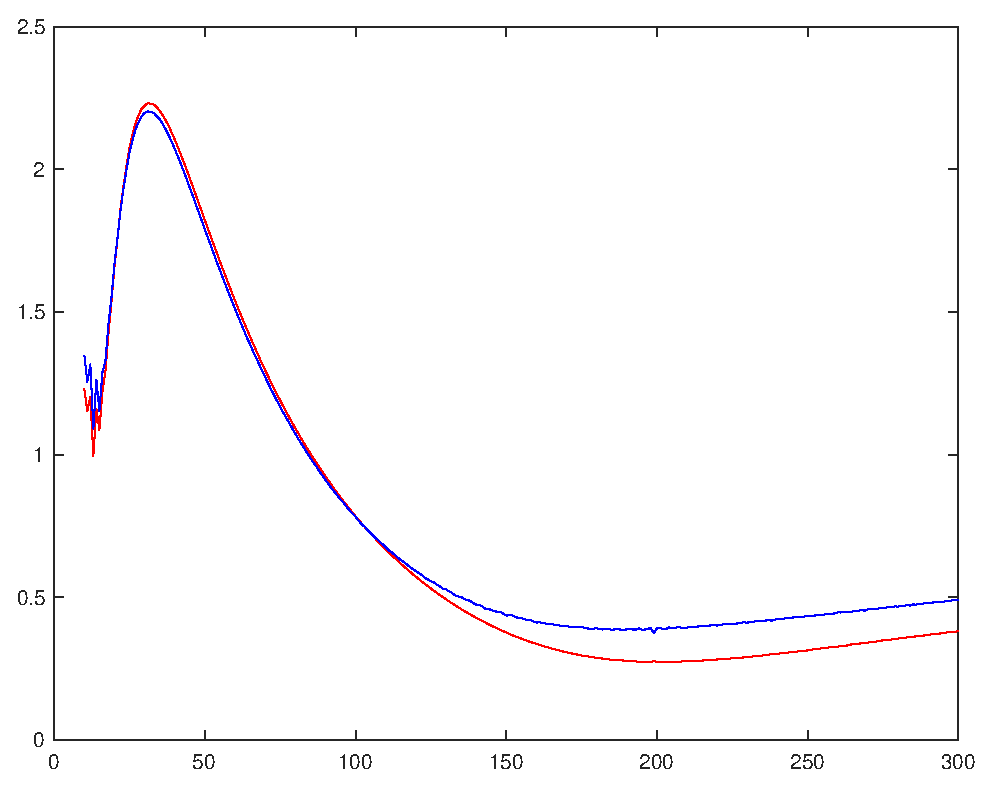
\includegraphics[width=0.4\textwidth]{ErrorBSplines.eps}
	\end{center}
	\caption{Fouten van de KKB implementatie.}
	\label{fig:errorkkb}
\end{figure}

\begin{figure}[H]
	\begin{center} 
		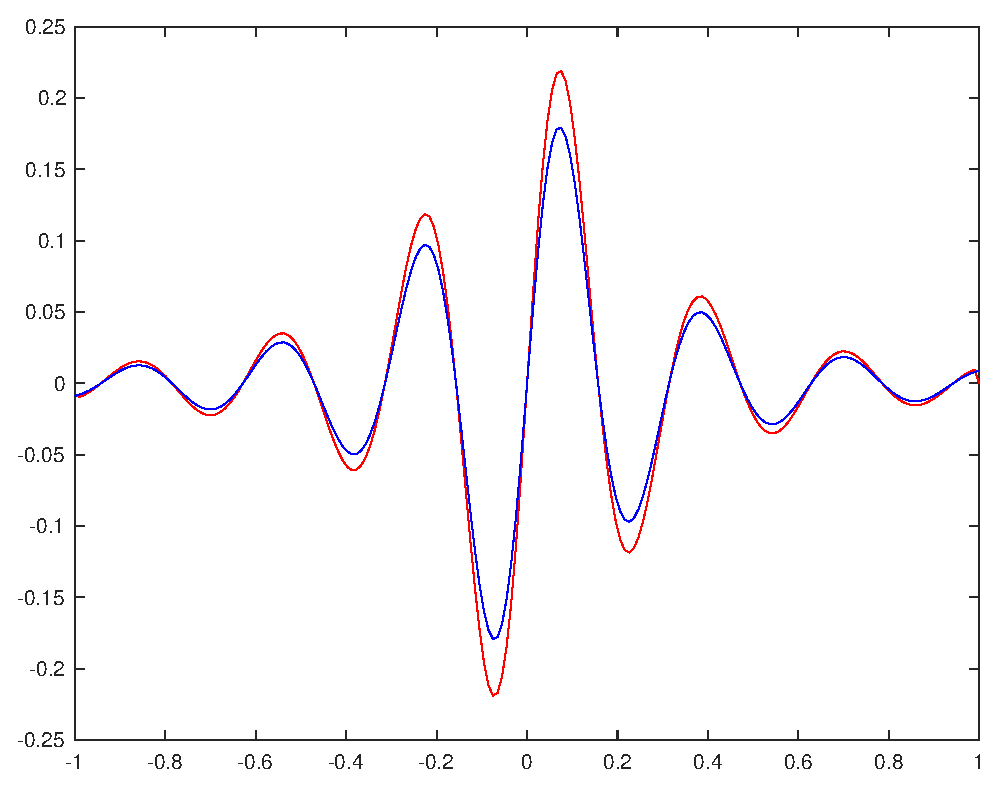
\includegraphics[width=0.4\textwidth]{PlotSplinesNoNoise.eps}
	\end{center}
	\caption{De functie f zonder ruis (rood) en beste benadering (blauw).}
	\label{fig:plotNoNoise}
\end{figure}

\begin{figure}[H]
	\begin{center} 
		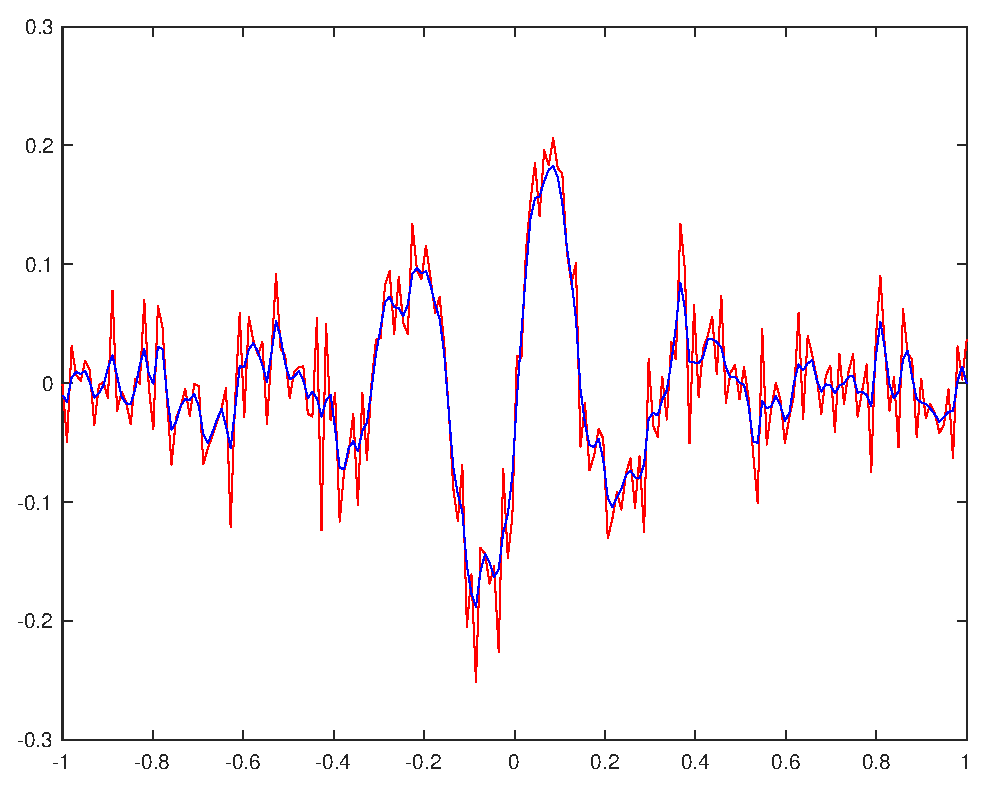
\includegraphics[width=0.4\textwidth]{PlotSplinesNoise.eps}
	\end{center}
	\caption{De functie f met ruis (rood) en beste benadering (blauw).}
	\label{fig:plotNoise}
\end{figure}

% Code 'n shit
\newpage
\section{Code}\label{sec:code}

% PDE code
\subsection{PDE Code}\label{sec:generalpde}

\subsubsection{PDE.m}\label{sec:pde}
\lstinputlisting[language=Matlab]{../Matlab/PDE.m}

\subsubsection{Opgave1.m}\label{sec:code1}
\lstinputlisting[language=Matlab]{../Matlab/opgave1.m}

\newpage
\subsubsection{Opgave2.m}\label{sec:code2}
\lstinputlisting[language=Matlab]{../Matlab/opgave2.m}

\subsubsection{Opgave3.m}\label{sec:code3}
\lstinputlisting[language=Matlab]{../Matlab/opgave3.m}

\newpage
\subsection{Spline Code}\label{sec:generalspline}

\subsubsection{KKB Spline}\label{sec:codekkb}
\lstinputlisting[language=Matlab]{../Matlab/kkbSpline.m}

\subsubsection{deBoor.m}\label{sec:codedb}
\lstinputlisting[language=Matlab]{../Matlab/deBoor.m}

\subsubsection{plotBSpline.m}\label{sec:codeplotb}
\lstinputlisting[language=Matlab]{../Matlab/plotBSpline.m}

\subsubsection{knotPoints.m}\label{sec:codeknot}
\lstinputlisting[language=Matlab]{../Matlab/knotPoints.m}

\subsubsection{binarySearch.m}\label{sec:codebinary}
\lstinputlisting[language=Matlab]{../Matlab/binarySearch.m}

\subsubsection{multiplicityKnotPoints.m}\label{sec:codemultiple}
\lstinputlisting[language=Matlab]{../Matlab/multiplicityKnotPoints.m}

\subsubsection{Opgave5.m}\label{sec:code5}
\lstinputlisting[language=Matlab]{../Matlab/opgave5.m}

\subsubsection{Opgave6.m}\label{sec:code6}
\lstinputlisting[language=Matlab]{../Matlab/opgave6.m}

\subsubsection{Opgave7.m}\label{sec:code7}
\lstinputlisting[language=Matlab]{../Matlab/opgave7.m}


\end{document}